%%%% Arquivo base para o documento - ver. 1.00 (24/02/2016)
% % % % % % % % % % % % % % % % 
% % % % % % % % % % % % % % % % 
%%%%%% MDT UFSM 2015 %%%%%%%%%%
% % % % % % % % % % % % % % % % 
% % % % % % % % % % % % % % % % 
% % %  OPÇÕES DE COMPILAÇÃO  %%%%%%%%%%%


% % % % % PAGINAÇÃO
% % % PAGINAÇÃO SIMPLES (FRENTE): PARA TRABALHOS COM MENOS DE 100 PAGINAS
\documentclass[oneside,openright,12pt]{ufsm_2015} %%%%% OPÇÃO PADRÃO -> PAGINAÇÃO SIMPLES. PARA TRABALHOS COM MAIS DE 100 PAGINAS COMENTE ESTA LINHA E DESCOMENTE A LINHA 
% % % % % % % % % % % % % % % % % % % % % % % % % % % % % % % % % % % % % % %
% PAGINAÇÃO DUPLA (FRENTE E VERSO): PARA TRABALHOS COM MAIS DE 100 PAGINAS
% \documentclass[twoside,openright,12pt]{ufsm_2015}  %%%% PARA MAIS DE 100 PAGINAS DESCOMENTAR
% % % % % % % % % % % % % % % % % % % % % % % % % % % % % % % % % % % % %

% % % % % % % % % % % % % % % % % % % % % % % % % % % % % % % % % % % % %
% % % % % % % % % % % % % % % % % % % % % % % % % % % % % % % % % % % % %
%%%%%%%%% DEFINIÇÃO PADRÃO DE PACOTES -- ALTERE POR SUA CONTA E RISCO
% % % % % % % % % % % % % % % % % % % % % % % % % % % % % % % % % % % % %

\usepackage{amsmath}
\usepackage{enumerate}
\usepackage{amssymb}
\usepackage{graphicx}
\usepackage{epsf,amsfonts}
\usepackage{amsfonts}
\usepackage{epstopdf}
\usepackage{float}
% % % %  PACOTE DE CODIFICAÇÃO - PADRÃO = UTF8
\usepackage[utf8]{inputenc}  %utf8
% \usepackage[latin1]{inputenc}   % europeu
% % % % % % % % % % % 
\usepackage[brazil]{babel}
\usepackage[T1]{fontenc}
\usepackage{indentfirst}
\usepackage{textcomp}
\usepackage{setspace}
\usepackage{picinpar}
\usepackage{ifthen}
\usepackage{path}
\usepackage{scalefnt}
\usepackage{tocloft}
\usepackage[overload]{textcase}

\usepackage{listings}


% % % % % % % % % % % % % % % % % % % % % % % % % % % % % % % % % % % % % % % % 
% % % % % % % % % % % FIM DA DEFINIÇÃO PADRÃO DE PACOTES  % % % % % % % % % % %
% % % % % % % % % % % % % % % % % % % % % % % % % % % % % % % % % % % % % % % % 

% % % % % % % % PACOTES PESSOAIS % % % % % % % %  

% Pacotes utilizados para gerar os gráficos.
\usepackage{comment}
\usepackage{subfigure}
\usepackage{tikz,pgfplots}
\usetikzlibrary{patterns}
% Configuração da área máxima que pode ser utilizada por imagem de gráfico.
\pgfplotsset{width=8cm,height=8cm,compat=1.8}

% % % % % %  DEFINIÇÕES PESSOAIS  


% % % % % % % % % % % % % % % % % % % % % % % % % % % % % % % % % % % % % % % %


% % % % % % % % % % % % % % % % % % % % % % % % % % % % % % % % % 
% % % % % % % % % % % % DADOS DO TRABALHO % % % % % % % % % % % % 
% % % % % % % % % % % % % % % % % % % % % % % % % % % % % % % % % 

% % % % % % % % % % INFORMAÇÕES INSTITUCIONAIS % % % % % % % % % % 
% % CENTRO DE ENSINO DA UFSM
\centroensino{Centro de Tecnologia}  %%% NOME POR EXTENSO
\centroensinosigla{CT}  %%% SIGLA

% % CURSO DA UFSM
\nivelensino{Graduação}  %%%%%%% NÍVEL DE ENSINO 
\curso{Sistemas de Informação}   %%%%% NOME POR EXTENSO
\ppg{PPGALGO}   %%%%%% SIGLAregister_error_handler
\statuscurso{Curso}  %%%% STATUS= {Programa} ou {Curso}


% % % % % % % % % % INFORMAÇÕES DO AUTOR % % % % % % % % % % 
\author{Lucas Lima de Oliveira}   %%%%% AUTOR DO TRABALHO
\sexo{M} %%%% SEXO DO AUTOR -> M=masculino   F=feminino (IMPORTANTE PARA AJUSTAR PAGINAS PRE-TEXTUAIS)
\grauensino{Graduação}    %%%%%%%% GRAU DE ENSINO A SER CONCLUÍDO
\grauobtido{Bacharel}    %%%%% TITULO OBTIDO
\email{loliveira@inf.ufsm.com.br}   %%%% E-MAIL PARA CATALOGRÁFICA (COPYRIGHT) - OBRIGATÓRIO
% \endereco{Nome da Rua, n. 999} %%%% ENDEREÇO PARA CATALOGRÁFICA (COPYRIGHT) - OPCIONAL
% \fone{11 2222 3333} %%%% TELEFONE PARA CATALOGRÁFICA (COPYRIGHT) FORMATO {11 2222 3333} - OPCIONAL
% \fax{11 2222 3333}  %%%% FAX PARA CATALOGRÁFICA (COPYRIGHT) FORMATO {11 2222 3333} - OPCIONAL


% % % % % % % % % % INFORMAÇÕES DA BANCA % % % % % % % % % % 
% OBSERVAÇÕES: O CAMPO ORIENTADOR É OBRIGATÓRIO E NÃO DEVE SER COMENTADO
% % % % % %    OS DEMAIS MEMBROS DA BANCA (COORIENTADOR E DEMAIS PROFESSORES) QUANDO COMENTADOS NÃO APARECEM NA FOLHA DE APROVAÇÃO (O LAYOUT DA FOLHA DE APROVAÇÃO ESTA PREPARADO PARA O ORIENTADOR E ATE MAIS 4 MEMBROS NA BANCA

\orientador{Sérgio Luís Sardi Mergen}{Dr}{UFSM}{M}{P}  %%%INFORMAÇÕES SOBRE ORIENTADOR: OS CAMPOS SÃO:{NOME}{SIGLA DA TITULAÇÃO}{SIGLA DA INSTITUIÇÃO DE ORIGEM}{SEXO} M=masculino F=feminino {PARTE DA BANCA?} P=presidente M=Membro  N=Não faz parte

% \coorientador{Coorientador}{Dr}{AAAA}{M}{M} %%%INFORMAÇÕES SOBRE CO-ORIENTADOR: OS CAMPOS SÃO:{NOME}{SIGLA DA TITULAÇÃO}{SIGLA DA INSTITUIÇÃO DE ORIGEM}{SEXO} M=masculino   F=feminino {PARTE DA BANCA?} P=presidente  M=Membro  N=Não faz parte

\bancaum{Joaquim Assuncao}{Dr}{UFSM}{M}{M}  %%%INFORMAÇÕES SOBRE PRIMEIRO NOME DA BANCA: OS CAMPOS SÃO:{NOME}{SIGLA DA TITULAÇÃO}{SIGLA DA INSTITUIÇÃO DE ORIGEM}{SEXO} M=masculino   F=feminino {PARTE DA BANCA?} P=presidente  M=Membro  N=Não faz parte

\bancadois{João Carlos Damasceno Lima}{Dr}{UFSM}  %%%INFORMAÇÕES SOBRE SEGUNDO NOME DA BANCA: OS CAMPOS SÃO:{NOME}{SIGLA DA TITULAÇÃO}{SIGLA DA INSTITUIÇÃO DE ORIGEM}

% \bancatres{Banca Três}{Dra}{CCCC} %%%INFORMAÇÕES SOBRE TERCEIRO NOME DA BANCA: OS CAMPOS SÃO:{NOME}{SIGLA DA TITULAÇÃO}{SIGLA DA INSTITUIÇÃO DE ORIGEM}

% \bancaquatro{Banca Quatro}{Dr}{DDDD} %%%INFORMAÇÕES SOBRE QUARTO NOME DA BANCA: OS CAMPOS SÃO:{NOME}{SIGLA DA TITULAÇÃO}{SIGLA DA INSTITUIÇÃO DE ORIGEM}

% \bancacinco{Banca Cinco}{Dra}{EEEE} %%%INFORMAÇÕES SOBRE QUARTO NOME DA BANCA: OS CAMPOS SÃO:{NOME}{SIGLA DA TITULAÇÃO}{SIGLA DA INSTITUIÇÃO DE ORIGEM}



% % % % % % % % % % INFORMAÇÕES SOBRE O TRABALHO % % % % % % % % % %
% % % %  TITULO DO TRABALHO
\titulo{Utilização de Algoritmos de Aprendizado de Máquina para Prever a Popularidade de Tuítes} %% NÃO EH NECESSÁRIO CAPITALIZAR

% % % %  TITULO DO TRABALHO EM INGLÊS
\englishtitle{Use of Machine Learning Algorithms to Predict Tweets Popularity}  %% NÃO EH NECESSÁRIO CAPITALIZAR

% % % ÁREA DE CONCENTRAÇÃO DO TRABALHO (CNPQ)
\areaconcentracao{Área de concentração do CNPq}
% % % TIPO DE TRABALHO - MANTER APENAS UMA LINHA DESCOMENTADA
% \tccg  %% Tese de <nível de ensino>
% \qualificacao %% Exame de Qualificação de <nível de ensino>
% \dissertacao %% Dissertação de <nível de ensino>
% \monografia %% Monografia
% \monografiag  %% Monografia (não exibe área de concentração)
% \tf  %% Trabalho Final de <nível de ensino>
% \tfg  %% Trabalho Final de Graduação (não exibe área de concentração)
% \tcc  %% Trabalho de Conclusão de Curso
\tccg  %% Trabalho de Conclusão de Curso (não exibe área de concentração)
% \relatorio  %% Relatório de Estágio (não exibe área de concentração)
% \generico   %%% Alternativa para aqueles cursos que não recebem o titulo de bacharel ou licenciado. Ex: engenharia, arquitetura, etc... Os campos abaixo também devem ser preenchidos
%     \tipogenerico{Tipo de trabalho em português}
%     \tipogenericoen{Tipo de trabalho em inglês}
%     \concordagenerico{o}
%     \graugenerico{Engenheiro Eletricista}
% % % DATA DA DEFESA 
\data{25}{12}{2018} %% FORMATO {DD}{MM}{AAAA}



% % % % %  ALGUMAS ENTRADAS PRE-TEXTUAIS
% % % % CASO NÃO QUEIRA UTILIZA-LAS COMENTE A LINHA DE COMANDO
% % % EPIGRAFE
\epigrafe{O livro é uma criatura frágil, ele sofre o desgaste do tempo, ele teme os roedores, os elementos e mãos desajeitadas. Então o livreiro proteje os livros não apenas da humanidade, mas também da natureza e devota sua vida a uma guerra contra as forças do esquecimento.}{Umberto Eco} %ESTRUTURA DE CAMPOS -> {Texto}{Autor}
% % % DEDICATÓRIA
\dedicatoria{Ao Rei da Espanha!}
% % % %  AGRADECIMENTOS
\agradecimentos{A mim!}

% % % % %  RESUMO E PALAVRAS CHAVE DO RESUMO - OBRIGATÓRIO PARA MDT-UFSM
\resumo{
Resumo aqui.
}
\palavrachave{Palavra Chave 1. Palavra 2. Palavra 3. (...)}
% "... deverão constar, no mínimo, três palavras-chave, iniciadas em
% letras maiúsculas, cada termo separado dos demais por ponto, e
% finalizadas também por ponto." MDT 2012

% % % % %  ABSTRACT E PALAVRAS CHAVE DO RESUMO - OBRIGATÓRIO PARA MDT-UFSM
\abstract{
Abstract here.
}
\keywords{Keyword 1. Keyword 2. Keyword 3. (...)}


% % %  ATIVAÇÃO DE LISTAS E PAGINAS ESPECIAIS
% % %  PARA QUE NÃO APAREÇAM NO TEXTO DESCOMENTE A LINHA ABAIXO -> POR PADRÃO TODAS ESTÃO ATIVIDADES

% % LISTA DE FIGURAS 
% \semfiguras   %%(QUANDO ATIVADA NÃO EXIBE A LISTA)
% % LISTA DE GRÁFICOS 
\semgraficos   %%(QUANDO ATIVADA NÃO EXIBE A LISTA)
% % LISTA DE ILUSTRAÇÕES 
\semilustracoes  %%(QUANDO ATIVADA NÃO EXIBE A LISTA)
% % LISTA DE TABELAS 
% \semtabelas   %%(QUANDO ATIVADA NÃO EXIBE A LISTA)
% % LISTA DE QUADROS 
\semquadros   %%(QUANDO ATIVADA NÃO EXIBE A LISTA)
% % LISTA DE APÊNDICES 
% \semapendices  %%(QUANDO ATIVADA NÃO EXIBE A LISTA)
% % LISTA DE ANEXOS 
% \semanexos   %%(QUANDO ATIVADA NÃO EXIBE A LISTA)



% % % %  LISTA DE ABREVIATURAS E SIGLAS
%%%%%%%% OBS: O espaço entre colchetes \item[] e um ambiente matemático
%%%%%%%% para não utilizar comente as linhas abaixo.
\siglamax{API} %%%% coloque aqui a maior sigla (indentação)
\listadeabreviaturasesiglas{
\item[API] \textit{Application Programming Interface}
\item[IA] \textit{Inteligência Artificial}
}

% % % %  LISTA DE SÍMBOLOS
%%%%%%%% OBS: O espaço entre colchetes \item[] e um ambiente matemático
%%%%%%%% para não utilizar comente as linhas abaixo.
% \simbolomax{(Re)2} %%%% coloque aqui o maior simbolo (indentação)
% \listadesimbolos{
% \item[u_*]	Escala de velocidade de fricção	
% \item[w_*]	Escala de velocidade convectiva
% \item[(Re)^2]	Maior simbolo da lista
% }


% % FICHA CATALOGRÁFICA
% \semcatalografica  %%%%  (QUANDO ATIVADA NÃO EXIBE A FICHA CATALOGRÁFICA NECESSITA DO ARQUIVO DA FICHA: ficha_catalografica.pdf

% % % A FICHA CATALOGRÁFICA FORNECIDA PELA UFSM EH UM PDF DO TAMANHO A4
% % % OS COMANDOS ABAIXO DEFINEM AS MARGENS PARA CORTAR A FICHA FORNECIDA E COLOCA-LA COMO UMA FIGURA NO DOCUMENTO LATEX
\margemesquerda{4}   %%%% CORTE DE MARGEM ESQUERDA EM CM
\margemdireita{1.5}   %%%% CORTE DE MARGEM DIREITA EM CM
\margemsuperior{17}  %%%% CORTE DE MARGEM SUPERIOR EM CM
\margeminferior{3} %%%% CORTE DE MARGEM INFERIOR EM CM
% % %  DICA: IMPRIMA UMA COPIA DA FICHA CATALOGRÁFICA E FACA A MEDIDA DAS MARGENS!


% % FOLHA DE ERRADA (versão rudimentar...pode ser aprimorado)
% % para não utilizar comente as linhas abaixo.
% % deve ser preenchida como um ambiente tabular de quatro colunas:
% % pagina & linha & onde se lê & leia-a se \\
%\errata{
%10   &    10    & errado   & certo \\
%\hline
%12    &    5     & errado com um texto mais longo & certo agora com um texto mais longo\\
%\hline
%13   &    3    & $x^2$   & $2x$\\
%}
% % % % % % % % % % % % % % % % % % % % % % % % % % % % % % % % % % % % % % % % % % % % % % 


% % % % % % % % % % % % % % % % % % % % % % % % % % % % % % % % % % % % % % 
% % % % % % % % % % % %  OPÇÕES DE FORMATAÇÃO % % % % % % % % % % % % % % %
% % % % % % % % % % % % % % % % % % % % % % % % % % % % % % % % % % % % % % 
% % % CAPITULO: por padrão alinhado a esquerda. Para ativar alinhamento centralizado descomente o comando abaixo

%\centralizado  %%%% <<< centraliza todos os capítulos

% % % % % % % % % % % % % % % % % % % % % % % % % % % % % % % % % % % % % %
% % % FONTES: descomente uma das opções. caso nenhuma seja ativada a classe usara a fonte padrão do latex

%% helvetica
% \usepackage[scaled]{helvet}
% \renewcommand*\familydefault{\sfdefault}

%% arial
\renewcommand{\rmdefault}{phv} % Arial
\renewcommand{\sfdefault}{phv} % Arial

%%times
% \usepackage{mathptmx}

% % % % % % % % % % % % % % % % % % % % % % % % % % % % % % % % % % % % % % 
% % % % % % % % % % % % % % % % % % % % % % % % % % % % % % % % % % % % % % 
% % % % % % % % % % % % % % % % % % % % % % % % % % % % % % % % % % % % % % 
% % % % % % % % % % % % % % % % % % % % % % % % % % % % % % % % % % % % % % 


% % % % % % % % % % % % % % % % % % % % % % % % % % % % % % % % % % % % % % 
% % % % % % % % % % % % % % % % % % % % % % % % % % % % % % % % % % % % % % 
% % % % % % % % % % % %  INICIO DO DOCUMENTO  % % % % % % % % % % % % % % %
% % % % % % % % % % % % % % % % % % % % % % % % % % % % % % % % % % % % % % 
% % % % % % % % % % % % % % % % % % % % % % % % % % % % % % % % % % % % % %


\begin{document}


% % % % % % % % % % % % % % % % % % % % % % % % % % % % % % % % % % % % % % 
\pretextual  %%%% GERA AS PAGINAS PRE-TEXTUAIS   
% % % % % % % % % % % % % % % % % % % % % % % % % % % % % % % % % % % % % % 

% % % % % % % % % % % % % % % % % % % % % % % % % % % % % % % % % % % % % % 
% % % % % CORPO DO TRABALHO - INCLUA OS SEUS TEXTOS AQUI
% % % % % SUGESTÃO -> UTILIZE ARQUIVOS EXTERNOS A PARTIR DO COMANDO \input


% % % % % % % % % % % % % % % % % % % % % % % % % % % % % % % % % % % % % % 
% % % % % % % % % % INICIO DAS PAGINAS TEXTUAIS % % % % % % % % % % % % % % 
% % % % % % % % % % % % % % % % % % % % % % % % % % % % % % % % % % % % % % 


% % % % % % % % % % % % % % % % % % % % % % % % % % % % % % % % % % % % % % 
% % % % % % % % % % % % % INTRODUÇÃO % % % % % % % % % % % % % % % % % % % % 
% % % % % % % % % % % % % % % % % % % % % % % % % % % % % % % % % % % % % % 
\introducao{

\par Com a grande popularização dos chamados influenciadores digitais, é notável o crescimento das mídias sociais como meios de comunicação e divulgação de conteúdos. Neste cenário, onde o número de seguidores determina a sua influência, torna-se muito importante que essas personalidades compreendam seu público, pois conteúdos direcionados refletem diretamente no alcance de suas publicações. Dentre as redes sociais mais utilizadas atualmente, o Twitter é um meio de veiculação de mensagens que se destaca, por sua simplicidade e objetividade. Embora não tenha o mesmo destaque que outras plataformas, como o Facebook ou o Instagram, o Twitter conta com cerca de 335 milhões de usuários ativos, segundo Statista~\footnote{\textit{Statista: }\texttt{https://www.statista.com/topics/737/twitter/}}, e em média 500 milhões de tuítes que são publicados diariamente, segundo \textit{Internet Live Stats}~\footnote{\textit{Internet Live Stats: }\texttt{http://www.internetlivestats.com/twitter-statistics/}}, o que faz dessa rede uma fonte de dados muito poderosa.

\par Uma das preocupações de usuários do Twitter é alavancar sua popularidade, através do aumento no número de seguidores. Essa preocupação é fundamental para empresas e personalidades públicas que utilizam suas imagens para fins monetários. Nesses casos, o uso das redes sociais deve ser planejado e monitorado. Quando isso é realizado da maneira correta, a marca e/ou a pessoa ficam muito mais próximos de seus fãs e seguidores, o que consequentemente, faz sua popularidade e influência aumentar. Como mencionado em \cite{artigo:oliveira:18}, um dos indicadores capaz de medir a influência de um usuário no Twitter, é a quantidade de retuítes que suas mensagens recebem, presente inclusive na fórmula para o cálculo de engajamento, o qual será explanado posteriormente. Considerando esse fator, pode-se afirmar empiricamente que o aumento na quantidade de retuítes leva a um aumento na quantidade de seguidores, devido a propagação exponencial daquele conteúdo.

\par Tendo em vista o interesse dos usuários em aumentar o alcance de suas postagens, poder identificar os fatores que têm maior influência sobre a popularidade de suas mensagens pode ser uma grande vantagem ao tentar aumentar o engajamento por parte de seus seguidores. Ser capaz de prever/estimar a popularidade que um tuíte poderá obter, baseando-se nas características presentes no corpo de sua mensagem, permite a realização de diferentes análises a cerca o conteúdo disseminado por aquela conta, o que pode trazer muitos benefícios aos usuários com relativa influência nessa rede social.

\par Como afirma \cite{ieee:suh:10}, a propagação de um tuíte está diretamente ligada ao conteúdo e valor informativo contido nele. Nesse sentido, os autores avaliaram um conjunto de características extraídas das mensagens. Os resultados mostraram que a utilização de \textit{hashtags} e URLs são fatores muito significativos e que ajudam a impulsionar uma publicação. Apesar de ser um resultado relevante, o trabalho não realizou uma análise exaustiva das características que podem ser extraídas das mensagens.

\par Dentro deste contexto, o objetivo deste trabalho é monitorar e extrair tuítes de determinadas contas do Twitter, a fim de elaborar um modelo, utilizando algoritmos de aprendizado de máquina, para realizar a predição e classificação da popularidade de tuítes com base em suas características. Devido ao grande volume de dados, faz-se necessário automatizar o processo de análise e classificação dos dados, para isso, serão estudados e testados algoritmos já consolidados, como Naive Bayes, J48 e LTM, contando inclusive com o auxílio de ferramentas já reconhecidas como Weka, para a aplicação e análise dos resultados destes algoritmos. Como entrada para estes algoritmos, serão utilizados dados provenientes do pré-processamento dos tuítes coletados, sendo consideradas três características que não foram contempladas pelo estudo de \cite{ieee:suh:10}: o tamanho em caracteres, o sentimento (que mede a emoção transmitida) e a banalidade (que mede a relevância da mensagem). Para fins de comparação, a presença de \textit{hashtags} e URLs também foi avaliada.

\par Este trabalho está estruturado nas seguintes seções. O capítulo \ref{sec:fund-teorica} apresenta a fundamentação teórica, abordando conceitos e algoritmos de aprendizado de máquina. O capítulo \ref{sec:trab-relacionados} apresenta os trabalhos relacionados. O capítulo \ref{sec:proposta} apresenta a definição dos atributo e a arquitetura de extração de tuítes usada, que realiza desde a coleta até a preparação dos dados para análise. O capítulo \ref{sec:experimentos} apresenta as análises realizadas a partir dos dados coletados juntamente com os algoritmos de aprendizado de máquina estudados. O capítulo \ref{sec:conclusao} apresenta as considerações finais a cerca do trabalho realizado.

}
% % % % % % % % % % % % % % % % % % % % % % % % % % % % % % % % % % % % % % 
\geraintro  %%%% GERA INTRODUÇÃO   % % % % % % % % % % % % % % % % % % % % % 
% % % % % % % % % % % % % % % % % % % % % % % % % % % % % % % % % % % % % % 
% % % % % % % % % % % % % % % % % % % % % % % % % % % % % % % % % % % % % % 

% % % % % % % % % % % % % % % % % % % % % % % % % % % % % % % % % % % % % % 
% % % % % % % % % % % % FUNDAMENTAÇÃO TEÓRICA  % % % % % % % % % % % % % % % 
% % % % % % % % % % % % % % % % % % % % % % % % % % % % % % % % % % % % % % 

\chapter{Fundamentação Teórica}
\label{sec:fund-teorica}

\par Neste capítulo serão apresentados os conceitos relacionados ao aprendizado de máquina, na seção \ref{sec:aprend-maquina}, definindo as diferenças entre a aprendizagem supervisionada e a não supervisionada. Em seguida, na seção \ref{sec:alg-aprend-maquina-sup}, são apresentados alguns dos principais algoritmos do segmento supervisionado, os quais também foram utilizados na realização de experimentos no decorrer deste trabalho, sendo estes o Naive Bayes, Árvores de Decisão e Redes Neurais.

% % % % % % % % APRENDIZADO DE MÁQUINA % % % % % % % %

\section{Aprendizado de Máquina}
\label{sec:aprend-maquina}

\par Entende-se como sistemas inteligentes, aqueles que são capazes de processar dados de entrada e ajustar padrões internos a fim de otimizar seus resultados de saída, de acordo com os objetivos esperados para aquele algoritmo. Dentro deste contexto, o aprendizado de máquina foca no treinamento desses algoritmos para melhorar seu desempenho. Esse processo está ligado com a redução de dimensionalidade, classificação e associação dos dados e previsão de comportamentos.

\par Algoritmos de aprendizado de máquina (ou \textit{machine learning} em inglês) dividem-se em dois segmentos, aqueles que necessitam de uma supervisão para melhorar seus resultados e aqueles fazem esse processo de maneira independente. Nesta seção serão apresentados esses dois tipos de algoritmos, especificando suas características e diferenças.

% % % % % % % % APRENDIZADO DE MÁQUINA SUPERVISIONADO % % % % % % % %

\subsection{Aprendizado de Máquina Supervisionado}
\label{sec:aprend-maquina-sup}

\par A aprendizagem supervisionada realiza o treinamento dos algoritmos com dados para os quais suas respostas já sejam conhecidas. Ou seja, dependem sempre da entrada de um padrão de valores e da comparação das respostas do sistema com aquelas consideradas corretas. Conforme o algoritmo é treinado seus padrões vão sendo ajustados a fim de diminuir o erro e otimizar as respostas. 

\par Os problemas solucionados através da aprendizagem supervisionada são divididos em problemas de regressão e classificação de dados, como ilustra a Figura \ref{fig:aprend-sup}. Segundo \cite{book:russell:10}, quando o resultado esperado pelo algoritmo for um conjunto finito de valores, (como fraco, mediano ou forte), trata-se de problema de classificação, pois os dados de entrada devem ser categorizados dentro daquele grupo. No caso do resultado esperado ser numérico, trata-se de um problema de regressão, na qual tenta-se identificar uma tendência nos valores com base nos dados de entrada.

\par Nesse tipo de aprendizagem o algoritmo recebe as entradas já categorizadas para realizar o treinamento e, a cada iteração, ajusta seus parâmetros para de obter a melhor saída, podendo ser, por exemplo, minimizar o erro, maximizar a precisão ou a acurácia. Frequentemente, após a etapa de treinamento, é realizada uma etapa de validação, passando ao algoritmo entradas sem classificação, dessa forma seu desempenho pode ser realmente avaliado e, se necessário, o treinamento pode ser realizado novamente com novos ajustes em seus parâmetros.

\pgfplotsset{compat=1.11}
\begin{figure}[!ht]
\caption{Exemplo de Problemas de Classificação e Regressão.}
\centering
\begin{tikzpicture}[scale=0.8]
	\begin{axis}[%
    	title={(a) Problema de Classificação},
    	scatter/classes={%
        	a={draw=blue, fill=blue, mark size=5}, 
        	b={mark=x, draw=red, fill=red, mark size=7, line width=3pt}
        }
    ]
    \addplot[scatter,only marks,%
        scatter src=explicit symbolic]%
        table[meta=label] {
        	x y label
        	1   2.5 a
            1.2 2   a
            1.5 4   a
            1.7 4.5 a
            2   3   a
            2.2 3.5 a
            2.5 1.6 a
            2.5 5.5 a
            2.7 4   a
            3   2.4 a
            3.1 3   a
            3.2 5   a
            3.9 2.1 a
            4   3.5 a
            5   2.4 a
            4.5 6.2 b
            5   5.1 b
            5.5 7.1 b
            6   4.3 b
            6.3 5.5 b
            6   6.2 b
            6.5 4.6 b
            7   3.5 b
            7   5.7 b
            7.1 7.2 b
            7.2 6.5 b
            7.5 5   b
            8.1 3.2 b
            8.2 4   b
            8.4 6   b
            8.6 5.5 b
    	};
    \draw [ultra thick, dotted, draw=brown] (9,0) -- (0,9);
	\end{axis}
\end{tikzpicture}
\hspace{0.25cm}
\begin{tikzpicture}[scale=0.8]
	\begin{axis}[%
    	title={(b) Problema de Regressão},
    	scatter/classes={%
        	a={draw=blue, fill=blue, mark size=5}, 
        	b={mark=x, draw=red, fill=red, mark size=7, line width=4pt}
        }
    ]
    \addplot[scatter,only marks,%
        scatter src=explicit symbolic]%
        table[meta=label] {
        	x y label
            1   2.5 a
            1.5 3.5 a
            2   3   a
            2.5 3.5 a
            2.7 4.5 a
            3   3   a
            3.5 4   a
            4   4.5 a
            4.5 3.7 a
            4.7 5.5 a
            5   4.5 a
            5.5 5   a
            6   6   a
            6.5 5.5 a
            7   6   a
            7.5 7.5 a
            8   7   a
            8.5 6.5 a
            9   8   a
    	};
    	\draw [ultra thick, dotted, draw=brown] (0,2) -- (10,8);
	\end{axis}
\end{tikzpicture}
\fonte{Produção do próprio autor.} % \citeonline{site:medium:pedro}
\label{fig:aprend-sup}
\end{figure}

% % % % % % % % APRENDIZADO DE MÁQUINA NÃO SUPERVISIONADO % % % % % % % %

\subsection{Aprendizado de Máquina Não Supervisionado}
\label{sec:aprend-maquina-nao-sup}

\par No caso dos algoritmos de aprendizagem não supervisionada, ao contrário do segmento apresentado na subseção anterior, estes recebem os dados sem nenhum classificação prévia, impossibilitando o aferimento das classes de cada entrada. Consequentemente, conforme os dados vão sendo recebidos, o próprio algoritmo é responsável por identificar as relações e padrões presentes nos dados, o que por si só pode ser considerado um objetivo a ser alcançado. A aprendizagem não supervisionada não prevê soluções específicas para realizar o treinamento e validação dos resultados, ou seja, não há um \textit{feedback} explícito sobre os resultados previstos.

Como explica \cite{book:russell:10}, o exemplo mais comum de aprendizagem não supervisionada, é o de agrupamento, onde o objetivo é detectar grupos potencialmente úteis dentro dos valores de entrada, que podem ser semelhantes ou estar relacionados por diferentes variáveis. A Figura \ref{fig:aprend-nao-sup} exemplifica as diferenças entre esses dois tipos de abordagem.

\pgfplotsset{compat=1.11}
\begin{figure}[!ht]
\caption{Exemplo da diferença entre as diferentes abordagens.}
\centering
\begin{tikzpicture}[scale=0.8]
	\begin{axis}[%
    	title={(a) Aprendizagem Supervisionada},
    	scatter/classes={%
        	a={draw=blue, fill=blue, mark size=5}, 
        	b={mark=x, draw=red, fill=red, mark size=7, line width=3pt}
        }
    ]
    \addplot[scatter,only marks,%
        scatter src=explicit symbolic]%
        table[meta=label] {
        	x y label
            1.7 2   a
            2.1 1.8 a
            2.1 2.3 a
            2.55 2.1 a
            2.1 2.05 a
            3.5 3.2 b
            3.8 3.5 b
            3.9 3.25 b
            4   3   b
            4.3 3.3 b
    	};
	\end{axis}
\end{tikzpicture}
\hspace{0.25cm}
\begin{tikzpicture}[scale=0.8]
	\begin{axis}[%
    	title={(b) Aprendizagem Não supervisionada},
    	scatter/classes={%
        	a={draw=blue, fill=blue, mark size=5}, 
        	b={mark=x, draw=red, fill=red, mark size=7, line width=4pt}
        }
    ]
    \addplot[scatter,only marks,%
        scatter src=explicit symbolic]%
        table[meta=label] {
        	x y label
            1.7 2   a
            2.2 1.8 a
            2.1 2.3 a
            2.55 2.1 a
            2.1 2.05 a
            3.5 3.2 a
            3.8 3.5 a
            3.9 3.25 a
            4   3   a
            4.3 3.3 a
    	};
	\end{axis}
	\draw[red, very thick] (1.4,1.4) circle (1.3);
	\draw[red, very thick] (5,5) circle (1.3);
\end{tikzpicture}
\fonte{Produção do próprio autor.} % \citeonline{site:medium:pedro}
\label{fig:aprend-nao-sup}
\end{figure}

% % % % % % % % ALGORITMOS DE APRENDIZADO DE MÁQUINA SUPERVISIONADO % % % % % % % %

\section{Algoritmos de aprendizado de máquina supervisionado}
\label{sec:alg-aprend-maquina-sup}

\par Dentro do escopo deste trabalho, que tem como um dos objetivos realizar a predição da popularidade de tuítes, requere-se a utilização da aprendizagem de máquina supervisionada, pois os resultados esperados estão diretamente ligados a classificação dos dados. Como mencionado, nesta seção serão abordados alguns dos principais algoritmos que se encaixam neste segmento e que serão utilizados no decorrer deste trabalho, apresentado suas características, funcionamento, vantagens e desvantagens na sua utilização.

% % % % % % % % NAIVE BAYES % % % % % % % %

\subsection{Naive Bayes}
\label{sec:naive-bayes}

\par A técnica Naive Bayes pode ser considerada como uma das mais populares para classificação de dados utilizando aprendizado de máquina. O algoritmo utiliza de métodos probabilísticos, baseados na Teoria Bayesiana, criada por Thomas Bayes no século XVIII. Para compreender melhor o funcionamento dessa técnica, é importante entender também um pouco sobre o teorema do qual ela teve origem.

\par Como mostra \cite{book:russell:10}, o teorema, ou regra de Bayes é uma formula simples, definida pela Equação \ref{eq:teorema-bayes}, que vem da regra do produto de probabilidades, assumindo que \textit{prob(D|H) = prob(H|D)}, sendo H a hipótese a ser validada e D os dados observados, podendo ser tratados também como \textit{causa} e \textit{efeito}. Apesar de simples, essa regra é a base de grande parte dos sistemas de IA (Inteligência Artificial) que utilizam inferência probabilística.
    
\begin{equation} \label{eq:teorema-bayes}
prob(H|D) = \frac{prob(D|H)prob(H)}{prob(D)}
\end{equation}

\par Dividindo as partes do teorema, do lado esquerdo, \textit{prob(H|D)} é chamada de probabilidade posterior da hipótese após a realização do experimento; do lado direito, \textit{prob(D|H)} chamada função de verossimilhança, é a distribuição de probabilidade dos dados, a qual multiplica-se por \textit{prob(H)}, denominada \textit{Prior}, que é a probabilidade da hipótese ser verdadeira; por fim, o denominador \textit{prob(D)}, é a probabilidade total.

\par Ainda que possa parecer um teorema simples, seu alcance está na sua capacidade de interpretação. No caso do modelo Naive Bayes, ou Bayes Ingênuo, assume-se que os atributos \textit{efeito} são condicionalmente independentes entre si, dada a \textit{causa} -- daí a denominação de ``ingênuo''. A distribuição probabilística deste modelo pode ser descrita conforme indica a Equação \ref{eq:naive-bayes}, sendo \textit{C} a classe, ou causa, que deve ser prevista, enquanto que o conjunto $\{x_1, ..., x_n\}$ são os atributos, ou efeitos.

\begin{equation} \label{eq:naive-bayes}
P(C | x_1, ..., x_n) = \alpha P(C)\prod_i{P(x_i | C)}
\end{equation}

\par Este modelo de aprendizagem é facilmente escalável para problemas maiores, funcionando muito bem com uma ampla variedade de aplicações, apesar de se destacar e ser comumente utilizado em uma série algoritmos para classificação de textos. Além disso, este modelo não apresenta grandes complicações com dados ruidosos ou faltantes, podendo inclusive realizar previsões adequadas nestes casos. Esses fatores fazem o Naive Bayes ser (provavelmente) o modelo de rede Bayesiana mais comumente utilizado em algoritmos de aprendizado de máquina.

\par Tomando como exemplo a clássica classificação de sentimentos em textos, como mencionado, o algoritmo irá assumir que as palavras de uma determinada mensagem não possuem uma relação entre si. Sendo assim, o classificador poderá presumir que uma frase seja positiva, caso a maioria das palavras presentes nela tenham maior probabilidade de ter este mesmo sentimento, independentemente do contexto em que foram utilizadas.

\par Para classificar uma determinada frase, inicialmente é preciso montar uma base de treinamento, contendo a classificação dos dados de entrada, que no caso da análise de sentimentos, será positivo ou negativo. A partir destes dados, é criada uma tabela para guardar a frequência de cada uma das entradas com suas classes e a probabilidades de cada entrada. Para testar uma nova entrada, é calculada sua probabilidade para cada uma das possíveis classificações com base nas ocorrências anteriores. Para os casos em que o dado de teste não está presente na base de treinamento ou não foi classificado para uma das classes, existem algumas técnicas capazes de corrigir esse problema. Uma técnica muito comum aplicada para estes casos é a suavização de Laplace, a qual soma o valor 1 para todos os valores, desta forma, nenhuma operação é realizada utilizando o valor 0.

\par Utilizando como exemplo a frase ``\textit{With great power comes great responsibility}'', e considerando a Tabela \ref{tab:naive-freq} (fictícia) apresentada logo abaixo, na qual consta a frequência das palavras para cada classe e a probabilidade de cada uma, para classificar a palavra ``\textit{great}'' como popular ou impopular, considerando também que essa possa ser uma frase extraída do Twitter, seriam realizadas as seguintes operações listadas a seguir.

\begin{table}[ht]
    \caption{Exemplo de tabela com frequências de palavras e suas classes.}
    \centering
    \begin{tabular}{ c c c c }
        \hline
        Palavras & Popular & Impopular & Probabilidade \\
        \hline
        responsibility & 1 & 2 & 3/14 = 0,21 \\
        power & 2 & 1 & 3/14 = 0,21 \\
        great & 3 & 1 & 4/14 = 0,28 \\
        bad & 0 & 2 & 2/14 = 0,14 \\
        good & 2 & 0 & 2/14 = 0,14 \\
        \hline
        Total & 8 & 6 & \\
        \hline
        & & Positivo & 8/14 = 0,57 \\
        & & Negativo & 6/14 = 0,42 \\
        \hline
    \end{tabular}
    \vspace{\baselineskip} %%% linha em branco para atender a norma
    \fonte{Produção do próprio Autor.}
    \label{tab:naive-freq}
\end{table}

\begin{align}
P(great|popular) = 3/8 = 0.37 \\
P(popular) = 8/14 = 0.57 \\
P(great) = 4/14 = 0.28 \\
P(great|unpopular) = 1/6 = 0.16 \\
P(unpopular) = 6/14 = 0.42
\end{align}

\begin{align}
P(popular|great) = 0.37 * 0.57 / 0.28 = 0.75 \\
P(unpopular|great) = 0.16 * 0.42 / 0.28 = 0.24
\end{align}

\par A partir dos cálculos realizados, com base na Tabela \ref{tab:naive-freq} apresentada, obtém-se como resultado uma probabilidade maior para a palavra `\textit{great}' ser popular. Para realizar a classificação considerando toda a frase, essa operação é aplicada para cada palavra, as probabilidades resultantes para cada classe são multiplicadas e os resultados são aplicados na regra de Bayes, conforme a Equação \ref{eq:teorema-bayes}, para cada uma das possíveis classes. Mesmo sendo um exemplo simples da aplicação da técnica Naive Bayes, é possível observar a facilidade da aplicação deste algoritmo para a classificação de dados utilizando um método probabilístico.

% % % % % % % % ÁRVORES DE DECISÃO % % % % % % % %

\subsection{Árvores de Decisão}
\label{sec:arvores-decisao}

% % % % % % % % REDES NEURAIS % % % % % % % %

\subsection{Redes Neurais} % Recorrentes
\label{sec:redes-neurais}

% % % % % % % % ENGENHARIA DE FEATURES % % % % % % % %

\subsection{Engenharia de \textit{Features}}
\label{sec:eng-features}

% % % % % % % % % % % % % % % % % % % % % % % % % % % % % % % % % % % % % % 
% % % % % % % % % % % % TRABALHOS RELACIONADOS % % % % % % % % % % % % % % % 
% % % % % % % % % % % % % % % % % % % % % % % % % % % % % % % % % % % % % % 

\chapter{Trabalhos Relacionados}
\label{sec:trab-relacionados}

% % % % % % % % % % % % % % % % % % % % % % % % % % % % % % % % % % % % % % 
% % % % % % % % % % % % % % % % PROPOSTA % % % % % % % % % % % % % % % % % % 
% % % % % % % % % % % % % % % % % % % % % % % % % % % % % % % % % % % % % % 

\chapter{Proposta}
\label{sec:proposta}

\par A proposta deste trabalho é a elaboração de um modelo, utilizando algoritmos de aprendizado de máquina supervisionada, capaz de classificar o nível de popularidade de tuítes com base na correlação entre a popularidade dos mesmos em função de um conjunto de características presentes no corpo das mensagens. Para atingir esse objetivo, é necessário coletar os tuítes, extrair suas características e aplicar o algoritmos já mencionados para realizar o treinamento e classificação dos dados. Esta seção apresenta a arquitetura de coleta e extração utilizada neste trabalho.

% % % % % % % % DEFINIÇÃO DOS ATRIBUTOS % % % % % % % %

\section{Definição dos Atributos}
\label{sec:def-atributos}

\par Como parte do objetivo deste trabalho é a correlação entre a popularidade e as características do texto de cada tuíte, é de fundamental importância a definição e extração de características relevantes que possam influenciar no interesse dos usuários sobre uma determinada mensagem. Esta etapa corresponde a definição dos atributos que serão extraídos de cada um dos tuítes coletados. Os itens abaixo definem cada um destes atributos e a razão de terem sido escolhidos:

\par \textbf{Presença de URLs}: Pode indicar uma informação proveniente de outros meios, podendo ser sites de notícias ou outras mídias sociais. Este fator pode despertar o interesse de usuários por um determinado tipo de informação.

\par \textbf{Presença de \textit{hashtags}}: De maneira geral, as \textit{hashtags} são palavras-chave ou termos utilizados para indicar que aquela mensagem está diretamente ligada a um tópico ou discussão específica. O que pode atrair o interesse de usuários por tópicos específicos, de maneira semelhante ao uso de URLs.

\par \textbf{Tamanho da mensagem}: O tamanho é basicamente a contagem da quantidade de caracteres usados no corpo do tuíte, que pode fazer com que os usuários percam ou não o interesse em ler seu conteúdo.

\par \textbf{Sentimento da mensagem:} O sentimento é um valor que classifica o teor do texto como positivo ou negativo. Fator que pode estar diretamente ligado a intenção de cada usuário em propagar mensagens com um determinado humor. Este atributo também pode chamado de polaridade da mensagem.

\par \textbf{Banalidade da mensagem:} No contexto deste trabalho, a banalidade corresponde à importância do que foi escrito no corpo do tuíte, levando em consideração a presença de palavras que são frequentemente usadas em textos escritos. Sendo assim, quanto maior o número de palavras frequentes, mais banal é a mensagem.

% % % % % % % % DEFINIÇÃO DE POPULARIDADE % % % % % % % %

\section{Definição de Popularidade}
\label{sec:def-popularidade}

\par Popularidade define-se por... Para calcular a taxa de engajamento em uma determinada publicação, por convenção, é realizada a fórmula apresentada na Equação \ref{eq:engajamento}. Cada elemento apresentado refere-se estritamente a quantidade obtida pela publicação. Trazendo para a realidade do Twitter, os compartilhamentos são substituídos pelos retuítes e os comentários pelas respostas a um determinado tuíte.

% retu\acute{\imath}tes
\begin{equation} \label{eq:engajamento}
E(x) = \frac{curtidas + compartilhamentos + coment\acute{a}rios}{seguidores}
\end{equation}

% % % % % % % % CLASSIFICADORES % % % % % % % %

\section{Classificadores}
\label{sec:classificadores}

\par Explicar que os classificadores utilizados para realização do trabalho foram Naive Bayes, árvores de decisão (quais algoritmos) e redes neurais recorrentes, com \textit{word embeddings (word2vec)}.

% % % % % % % % % % % % % % % % % % % % % % % % % % % % % % % % % % % % % % 
% % % % % % % % % % % % % % EXPERIMENTOS  % % % % % % % % % % % % % % % % % 
% % % % % % % % % % % % % % % % % % % % % % % % % % % % % % % % % % % % % % 


\chapter{Experimentos}
\label{sec:experimentos}

\section{Extração de Tuítes}
\label{sec:extracao-tweets}

\par A arquitetura, exibida na Figura~\ref{fig:arquitetura}, tem os seguintes módulos: (a) \textbf{Coleta} dos tuítes publicados por cada uma das contas acompanhadas; (b) \textbf{Extração} das características de cada tuíte; e (c) \textbf{Atualização} periódica dos dados coletados.

\begin{figure}[ht]
    \caption{Arquitetura adotada para extração de tuítes}
    \centering
    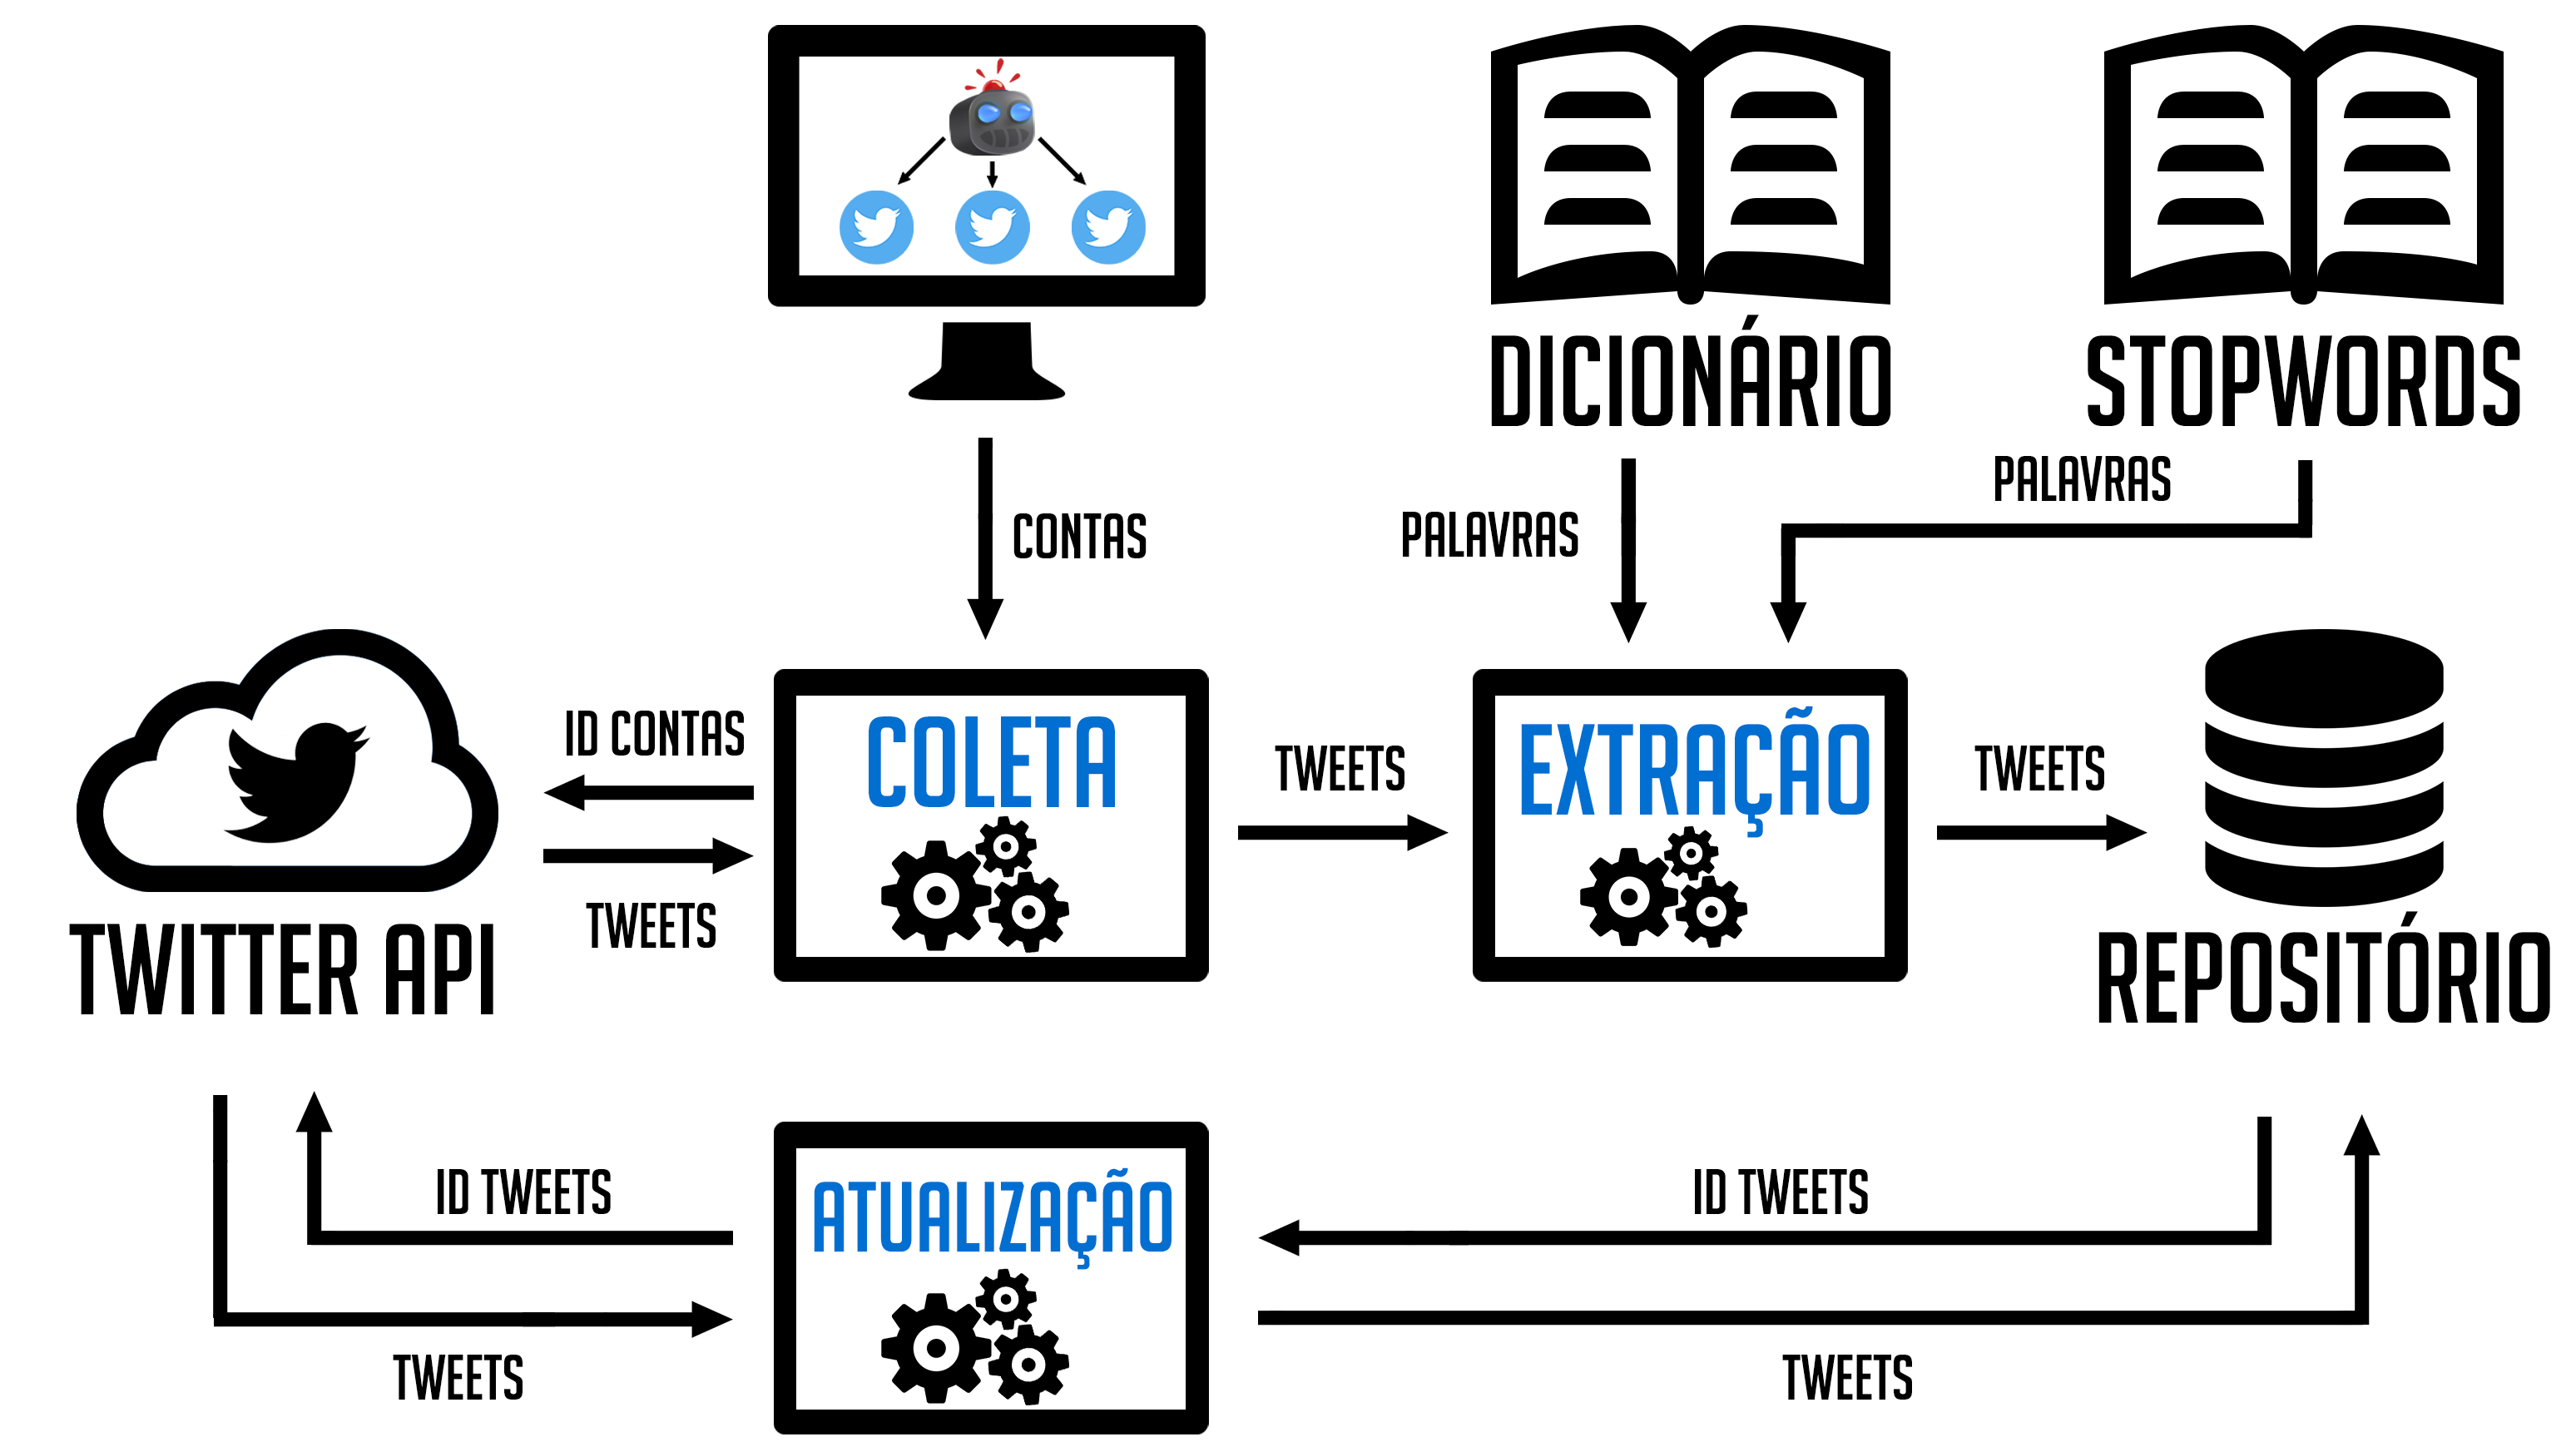
\includegraphics[width=1\textwidth]{figuras/arquitetura.png}
    \vspace{\baselineskip} %%% linha em branco para atender a norma
    \fonte{Produção do próprio autor.}
    \label{fig:arquitetura}
\end{figure}

% % % % % % % % COLETA DE TUÍTES % % % % % % % %
\subsection{Coleta de tuítes}

\par O módulo de coleta é responsável por extrair tuítes de usuários específicos. A extração ocorre de forma contínua, usando recursos de \textit{streaming} disponibilizados pela API do Twitter\footnote{\textit{Twitter Developer Platform:} \texttt{https://dev.twitter.com}}. São coletados todos tuítes publicados a partir do momento que o \textit{streaming} entra em execução.

\par A especificação das contas a serem seguidas é feita a partir de uma conta raiz. São extraídos os tuítes publicados em inglês por todos usuários seguidos por essa conta raiz. Essa estratégia permite que novas contas sejam adicionadas à lista sem que haja interrupções na execução do algoritmo. O módulo também conta com tratamento de exceções para que a coleta não seja interrompida devido à problemas temporários de acesso aos dados, como indisponibilidade do serviço ou extrapolação do limite de requisições permitido por instante de tempo.

\par Na Tabela \ref{tab:dados-coleta} podem ser visualizadas as informações extraídas de cada tuíte através da API. O campo ``mensagem'' é usado para a extração das características. Já os campos ``seguidores'', ``retuítes'' e ``curtidas'' são usados cálculo para medir a taxa de engajamento de cada tuíte\footnote{Infelizmente a API do Twitter permite a extração da quantidade de respostas apenas na versão paga, impossibilitando a contabilização desse valor na fórmula de engajamento.}. Por sua vez, os campos ``identificação'' e ``data/hora'' são usados pelo módulo de atualização.

\begin{table}[ht]
\centering
\caption{Dados coletados para cada tuíte}
\label{tab:dados-coleta}
\begin{tabular}{|l|l|}
\hline
\textbf{Informação} & \textbf{Conteúdo} \\ \hline
autor               &  código e nome da conta que originou o tuíte \\ \hline
seguidores          &  quantidade de seguidores da conta que originou o tuíte \\ \hline
identificação       & código do tuíte (permite a consulta posterior) \\ \hline
mensagem            & texto de no máximo 280 caracteres \\ \hline
data e hora         & data e hora da publicação do tuíte em seu país de origem \\ \hline
retuítes            & quantidade de retuíte que a mensagem recebeu \\ \hline
curtidas            & quantidade de vezes que o tuíte foi favoritado \\ \hline
\end{tabular}
\end{table}

% % % % % % % % EXTRAÇÃO DAS CARACTERÍSTICAS % % % % % % % %
\subsection{Extração das Características}

\par Esta etapa corresponde a extração das características de cada um dos tuítes coletados. A extração ocorre imediatamente após a coleta. Os itens abaixo mostram como cada característica foi extraída:

\par \textbf{Presença de URLs e \textit{hashtags}}: O uso desses recursos na mensagem é facilmente detectado pela presença de prefixos específicos no corpo da mensagem. Por exemplo, o prefixo ``http'' indica que URLs foram usadas, enquanto que o prefixo ``\#'' denota o uso de \textit{hashtags}. 

\par \textbf{Tamanho da mensagem}: O tamanho é extraído através da contagem da quantidade de caracteres presentes no texto. A contagem desconsidera caracteres usados em URLs, assumindo que \textit{hiperlinks} não transmitam nenhuma mensagem.  A remoção de URLs foi realizada a partir da aplicação de uma expressão regular.

%%%%%%%%%%%%%%% EXTRAÇÃO DO SENTIMENTO %%%%%%%%%%%%%%%
\par \textbf{Extração do sentimento:} Para realizar a extração do sentimento, foi utilizada a biblioteca TextBlob da linguagem Python \cite{loria:14}. Essa biblioteca  permite a obtenção da polaridade e subjetividade de conteúdos textuais na língua inglesa. A API também fornece a possibilidade de tradução do conteúdo de textos escritos em outras linguagens.
% assim como no trabalho de \cite{engel:16}

\par A extração do sentimento realizada pela biblioteca se baseia em Árvores de Decisão e no modelo de classificação \textit{Naive Bayes} -- ambos já apresentados na seção \ref{sec:fund-teorica} --, o que elimina a necessidade de elaborar no novo algoritmo para realizar essa função. A classificação da mensagem retorna um valor decimal entre o intervalo de -1 e 1, onde -1 corresponde a uma mensagem totalmente negativa, 0 corresponde a neutra e 1 corresponde a totalmente positiva. 

%%%%%%%%%%%%%%% EXTRAÇÃO DA BANALIDADE %%%%%%%%%%%%%%%
\par \textbf{Extração da banalidade:} A forma adotada para medir a banalidade considerando o uso de palavras comuns em textos escritos, utiliza a Equação \ref{eq:banalidade}, apresentada logo abaixo.

\begin{equation} \label{eq:banalidade}
\frac{\sum_{i=1}^n (freq(P_i))}{n}
\end{equation}

\par onde o conjunto $\{P_1, ..., P_n\}$ são as palavras da mensagem após a remoção de \textit{stopwords} (preposições e artigos que normalmente são descartados durante o processamento de um texto). Já a função $freq(P)$ retorna 1 caso a palavra $P$ seja frequente e zero caso não seja. A verificação da frequência utiliza um dicionário contendo 3000 palavras comuns da língua inglesa\footnote{\textit{3000 most common words in English: }\texttt{https://www.ef.com/english-resources/ english-vocabulary/top-3000-words/}}. Também são removidas as \textit{hashtags} e menções a outros usuários, por entender que não se tratam de palavras que podem ser caracterizadas como banais ou não.

\par Na Tabela \ref{tab:dados-extracao} pode ser visto um exemplo geral de todas as caraterísticas extraídas nesta etapa.

\begin{table}[ht]
\centering
\caption{Dados obtidos na etapa de Extração}
\label{tab:dados-extracao}
\begin{tabular}{|l|l|}
\hline
\textbf{Informação} & \textbf{Conteúdo} \\ \hline
sentimento			& valor entre -1 e 1 correspondente a polaridade do texto \\ \hline
URL					& valor 1 se houver URL no texto e 0 se não houver \\ \hline
\textit{hashtag} 	& valor 1 se houver \textit{hashtag} no texto e 0 se não houver \\ \hline
tamanho 			& quantidade de caracteres utilizados na mensagem \\ \hline
banalidade			& somatório baseado na no uso de palavras frequentes \\ \hline
\end{tabular}
\end{table}


% % % % % % % % ATUALIZAÇÃO DOS DADOS % % % % % % % %
\subsection{Atualização dos dados de retuítes e curtidas}

\par Como o módulo de coleta funciona por meio de \textit{streaming}, os tuítes são coletados no instante de sua criação. Nesse momento, a quantidade de retuítes e curtidas recebidos têm o valor zero. Dessa forma, é necessária uma conferência periódica para a obtenção dos dados atualizados.

\par A atualização é realizada através de um recurso da API do Twitter que obtém informações de um tuíte a partir do seu código de identificação. Para evitar sobrecarga de processamento, apenas os tuítes publicados no intervalo de 15 dias são atualizados. Como os dados de tuítes mais antigos raramente são modificados, a busca para a atualização de cada um deles seria ao mesmo tempo custosa e improdutiva.

% % % % % % % % % % % % % % % % % % % % % % % % % % % % % % % % % % % % % % 
% % % % % % % % % % % % % % % CONCLUSÕES % % % % % % % % % % % % % % % % % %
% % % % % % % % % % % % % % % % % % % % % % % % % % % % % % % % % % % % % % 

\chapter{Conclusões}
\label{sec:conclusao}


% % % % % % % % % % % % % % % % % % % % % % % % % % % % % % % % % % % % % % 
% % % % % % % % % % % % FIM DAS PAGINAS TEXTUAIS % % % % % % % % % % % % % % 
% % % % % % % % % % % % % % % % % % % % % % % % % % % % % % % % % % % % % % 


% % % % % % % % % % % % % % % % % % % % % % % % % % % % % % % % % % % % % % 	
% % % % % % % % % % % % % BIBLIOGRAFIA  % % % % % % % % % % % % % % % % % % 
% % % % % % % % % % % % % % % % % % % % % % % % % % % % % % % % % % % % % % 	

\bibliografia{referencias}  %%%%% BIBLIOGRAFIA -> INCLUIR NAS CHAVES O NOME DO ARQUIVO *.BIB	
	
% % % % % % % % % % % % % % % % % % % % % % % % % % % % % % % % % % % % % 	
% % % % % % % % % % % % % APÊNDICES % % % % % % % % % % % % % % % % % % %
% % % % % % % % % % % % % % % % % % % % % % % % % % % % % % % % % % % % % 	
\apendice %%%% TEXTOS A PARIR DESTE PONTO SERÃO CONSIDERADOS APÊNDICES

\chapter{Demonstração de algo}
\label{sec:apendice-demonst-algo}
        \par Algo como apêndice.  
        
% % % % % % % % % % % % % % % % % % % % % % % % % % % % % % % % % % % % % % 	
% % % % % % % % % % % % % % % ANEXOS  % % % % % % % % % % % % % % % % % % % 
% % % % % % % % % % % % % % % % % % % % % % % % % % % % % % % % % % % % % % 	
\anexo    %%%% TEXTOS A PARIR DESTE PONTO SERÃO CONSIDERADOS ANEXOS

\chapter{Algo interessante que alguém fez}
\label{sec:anexo-algo-interessante}
         \par Algo como anexo.

\end{document}

